% http://www.texample.net/tikz/examples/tree/
\documentclass[border=10pt]{standalone}
\usepackage{tikz}
\begin{document}

%\tikzset{level1/.style={sibling distance=5em};}
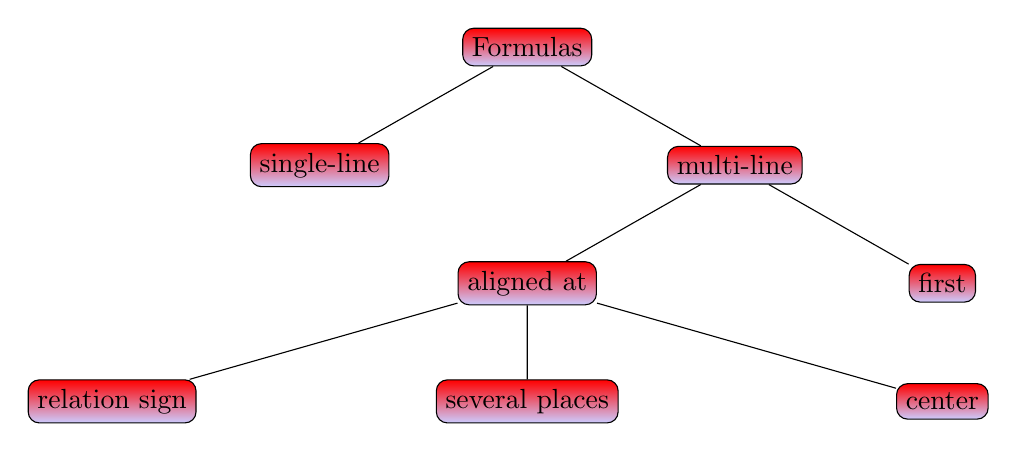
\begin{tikzpicture}[sibling distance=15em,
  every node/.style = {shape=rectangle, rounded corners,
    draw, align=center,
    top color=red, bottom color=blue!20}]]
  \node {Formulas}
    child { node {single-line} }
    child { node {multi-line}
      		child { node {aligned at}
        			child { node {relation sign} }
        			child { node {several places} }
        			child { node {center} } 
			}
      		child { node {first} } 
      };
\end{tikzpicture}
\end{document}

[sibling distance=10em,
  every node/.style = {shape=rectangle, rounded corners,
    draw, align=center,
    top color=white, bottom color=blue!20}]]